\begin{figure*}[tb]
\centering
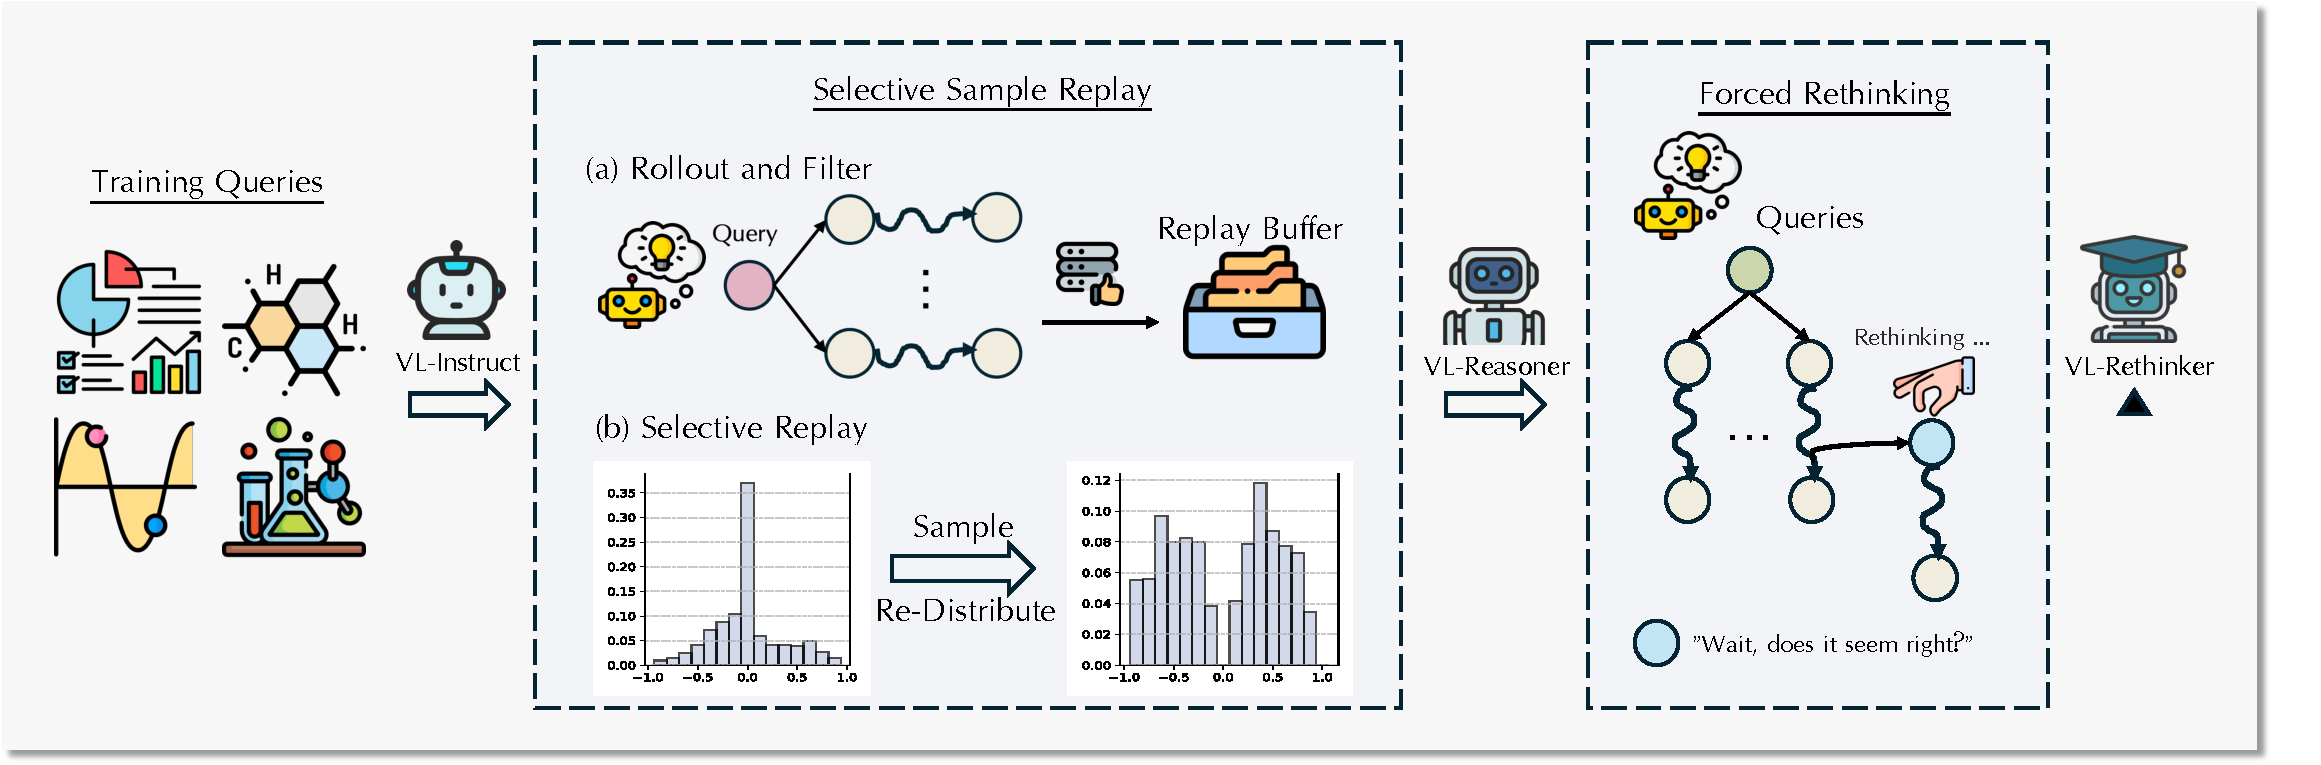
\includegraphics[width=\textwidth]{figures/overview-2.pdf}
\caption{\small \textbf{Method overview.} Starting from an instruction-tuned VLM (VL-Instruct), RL with Selective Sample Replay (SSR) produces VL-Reasoner: (a) rollouts for each query are scored with a binary correctness reward and samples with non-zero advantage are kept in a replay buffer; (b) replay samples from the buffer with priority increasing in $|$advantage$|$, redistributing the training batch away from the spike at zero advantage (left histogram) towards informative samples (right histogram). Forced Rethinking then appends a rethinking trigger (e.g., ``Wait, does it seem right?'') to a fraction of rollouts during RL, yielding \model.}
\label{fig:overview}
\end{figure*}
